\documentclass{article}\usepackage[]{graphicx}\usepackage[]{color}
%% maxwidth is the original width if it is less than linewidth
%% otherwise use linewidth (to make sure the graphics do not exceed the margin)
\makeatletter
\def\maxwidth{ %
  \ifdim\Gin@nat@width>\linewidth
    \linewidth
  \else
    \Gin@nat@width
  \fi
}
\makeatother

\definecolor{fgcolor}{rgb}{0.345, 0.345, 0.345}
\newcommand{\hlnum}[1]{\textcolor[rgb]{0.686,0.059,0.569}{#1}}%
\newcommand{\hlstr}[1]{\textcolor[rgb]{0.192,0.494,0.8}{#1}}%
\newcommand{\hlcom}[1]{\textcolor[rgb]{0.678,0.584,0.686}{\textit{#1}}}%
\newcommand{\hlopt}[1]{\textcolor[rgb]{0,0,0}{#1}}%
\newcommand{\hlstd}[1]{\textcolor[rgb]{0.345,0.345,0.345}{#1}}%
\newcommand{\hlkwa}[1]{\textcolor[rgb]{0.161,0.373,0.58}{\textbf{#1}}}%
\newcommand{\hlkwb}[1]{\textcolor[rgb]{0.69,0.353,0.396}{#1}}%
\newcommand{\hlkwc}[1]{\textcolor[rgb]{0.333,0.667,0.333}{#1}}%
\newcommand{\hlkwd}[1]{\textcolor[rgb]{0.737,0.353,0.396}{\textbf{#1}}}%
\let\hlipl\hlkwb

\usepackage{framed}
\makeatletter
\newenvironment{kframe}{%
 \def\at@end@of@kframe{}%
 \ifinner\ifhmode%
  \def\at@end@of@kframe{\end{minipage}}%
  \begin{minipage}{\columnwidth}%
 \fi\fi%
 \def\FrameCommand##1{\hskip\@totalleftmargin \hskip-\fboxsep
 \colorbox{shadecolor}{##1}\hskip-\fboxsep
     % There is no \\@totalrightmargin, so:
     \hskip-\linewidth \hskip-\@totalleftmargin \hskip\columnwidth}%
 \MakeFramed {\advance\hsize-\width
   \@totalleftmargin\z@ \linewidth\hsize
   \@setminipage}}%
 {\par\unskip\endMakeFramed%
 \at@end@of@kframe}
\makeatother

\definecolor{shadecolor}{rgb}{.97, .97, .97}
\definecolor{messagecolor}{rgb}{0, 0, 0}
\definecolor{warningcolor}{rgb}{1, 0, 1}
\definecolor{errorcolor}{rgb}{1, 0, 0}
\newenvironment{knitrout}{}{} % an empty environment to be redefined in TeX

\usepackage{alltt}
\usepackage{amsmath}
\usepackage{makecell}
\setcellgapes{5pt}
\usepackage{graphics}
\usepackage{multirow}
\usepackage{multicol}
\usepackage[cm]{fullpage}
\graphicspath{ {./images/} }
\usepackage{titling}
\usepackage[table]{xcolor}
\usepackage[mathscr]{euscript}
\usepackage{mathrsfs}
\usepackage{ulem, cancel}
\usepackage{boldline}

\title{COSC 6323 - Statistical Methods in Research\\Project Phase - 2\\}

\author{%
    Members: Team-8 \\\\
    1. Farah Naz Chowdhury,    \texttt{ID:1798957}, \texttt{fchowdhury4@uh.edu}      \vspace{2pt} \\
    2. Md Rafiqul Islam Rabin, \texttt{ID:1797648}, \texttt{mrabin@central.uh.edu}   \vspace{2pt} \\
    3. S M Salah Uddin Kadir , \texttt{ID:1800503}, \texttt{ssalahuddinkadir@uh.edu} \vspace{2pt} \\
}

\date{April 05, 2019.}
\IfFileExists{upquote.sty}{\usepackage{upquote}}{}
\begin{document}

\maketitle
\par{\textbf{Contributions}: We sit together several times to discuss about the requirement and task distribution. Fortunately, there was no task break down needed as we agreed to sit together to implement the tasks (i.e. data, figure, model and table) equally. So, the contribution status - Fig 4 (Salah, Rabin, Prity), Table S2 (Rabin, Prity, Salah) and Table S3 (Rabin, Prity, Salah). We always shared our progress/problem with each other and helped during implementation. We distributively contributed to our created git repository for the project. As we all completed our tasks and actively involved with each other all the times, we equally contributed to this phase of the project.}

%Fig. 4
\newpage
\section*{\underline{Fig. 4:}}
\begin{center}
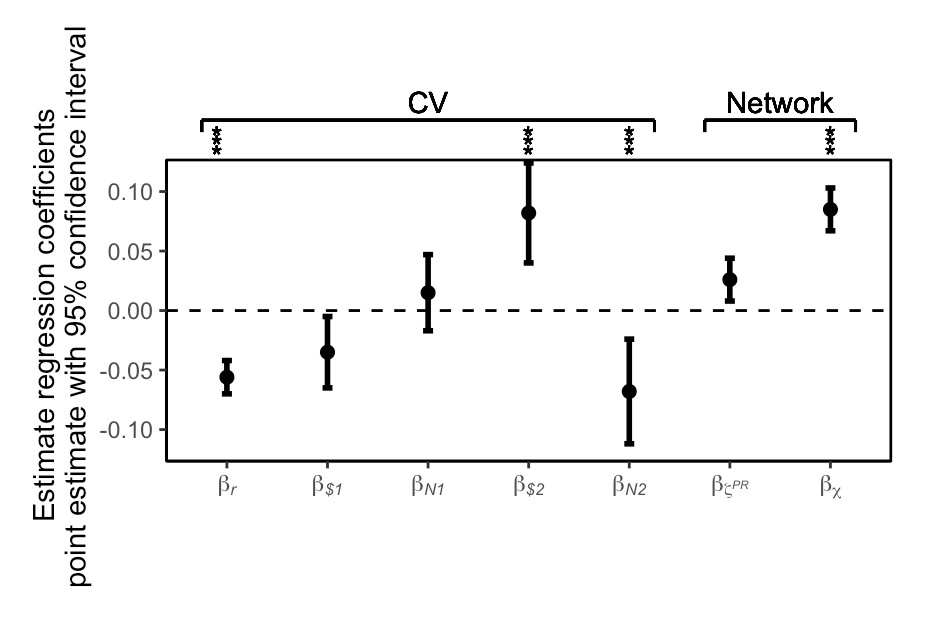
\includegraphics[scale=1.0]{Fig4.png}
\newline
\par{\textbf{Fig. 4. Career cross-sectional regression model.}}
\end{center}
\subsection*{\underline{Description of figure content:}}
\par{
The figure shows the standardized coefficient values of (CV + Network) model. Each coefficient values has corresponding error ranges and split into two groups: researchers's CV and collaboration network. We have specified the CV coefficients and Network coefficients using the annotation. We have used the three star (***) annotation to specify the coefficients which probability of $p-value$ is as follows: ***$\textit{p}$ $\leq$ .001.
}
\subsection*{\underline{Observations, conclusions, and hypotheses:}}
\par{
From the figure, we can see that the total amount of funding ($\beta_{\$2}$) of NIH is greater than the total amount of NSF funding ($\beta_{\$1}$). The $p-value$ of NIH is less than $0.001$ which indicates the NIH coefficients are significant. Although, the correlation with the number of NIH grants ($\beta_{N2}$) is negative, so the cost is related to the management of several smaller grants versus fewer bigger grants. On the other hand, the $p-values$ of NSF coefficients are greater than 0.001, so we can say that the estimates of NSF variables are not significant in the OLS model. Therefore, there is different levels of dependency on the NIH/NSF funding between the biology and computer science faculty. The main result of this plot shows that the higher degrees of cross-disciplinary activity $(\beta_{\chi} > 0, P < 0.001)$ correlate with the higher career citations.
}

%Table S2
\newpage
\section*{\underline{Table S2:}}
\begin{table}[h!]
  \begin{center}
  \resizebox{\columnwidth}{!}{%
  \begin{tabular}{l l c l c l c}
  \hline \hline
  {} &
  \multicolumn{2}{c}{\textbf{CV}} &
  \multicolumn{2}{l}{\textbf{CV + Network}} &
  \multicolumn{2}{c}{\textbf{CV + Network [Standardized]}} \\
  \hline
  \textbf {CV parameters} \\
  Departmental rank, $\beta_{r}$
  & -0.052*** & (0.006) & -0.047*** & (0.006) & -0.056*** & (0.007) \\
  Productivity (\textit{h}-index), $\beta_{h}$
  & 1.857***  & (0.016) & 1.866***  & (0.018) & 1.179***  & (0.012) \\
  Total NSF funding, $\beta_{\$1}$
  & -0.005*   & (0.002) & -0.005*   & (0.002) & -0.035*   & (0.015) \\
  {\#} of NSF grants, $\beta_{N1}$
  & 0.024     & (0.014) & 0.013     & (0.015) & 0.015     & (0.016) \\
  Total NIH funding, $\beta_{\$2}$
  & 0.016***  & (0.004) & 0.014***  & (0.003) & 0.083***  & (0.021) \\
  {\#} of NIH grants, $\beta_{N2}$
  & -0.067*** & (0.019) & -0.061*** & (0.019) & -0.069*** & (0.022) \\
  \hline
  \textbf {Network parameters}\\
  PageRank Centrality, $\beta_{\mathscr{C}^{PR}}$
  &           &         & 0.041**   & (0.014) & 0.026**   & (0.009) \\ 
  Cross-disciplinarity, $\beta_{x}$
  &           &         & 0.571***  & (0.061) & 0.086***  & (0.009) \\ 
  \hline
  Discipline ($\mathscr{O}$) dummy
  & Y         &         & Y         &         & Y         &         \\
  5-year cohort $(y{^0_{i,5}})$ dummy
  & Y         &         & Y         &         & Y         &         \\
  Constant
  & 1.398***  & (0.234) & 1.706***  & (0.271) &  7.744*** & (0.216) \\
  \hline
  $\textit{n}$
  & 4190      &         & 3900      &         & 3900      &         \\
  adj. ${R^2}$
  & 0.883     &         & 0.882     &         & 0.882     &         \\
  \hline \hline
  Standard errors in parentheses.
  & & \quad\quad\quad\quad\quad\quad\quad\quad\quad\quad 
  & & \quad\quad\quad\quad\quad\quad\quad\quad\quad\quad 
  & & \\
  {* $\textit{p}$ $\leq$ .05, ** $\textit{p}$ $\leq$ .01, *** $\textit{p}$ $\leq$ .001}
  &           &         &           &         &           &         \\
  \end{tabular}%
  }
  \end{center}
\end{table}
\begin{center}
\par{\textbf{Table S2. Career data set: Pooled cross-sectional model.}}
\end{center}
\subsection*{\underline{Description of figure content:}}
\par{
The following is the cross-sectional ordinary least squares (OLS) regression model:
\\\\ $lnC_i = {{\beta}_r}ln{r_i} + {{\beta}_h}ln{h_i} + {{\beta}_{\$1}}ln{{\$_i}^{NSF}} + {{\beta}_{N1}}ln{{N_i}^{NSF}} + {{\beta}_{\$2}}ln{{\$_i}^{NIH}} + {{\beta}_{N2}}ln{{N_i}^{NIH}} + {{\beta}_{\mathscr{C}}}ln{{\mathscr{C}_i}^{PR}} + {{\beta}_{\chi}}{{\chi}_i} + D(O(\mathcal{F}_i)) + D(y_{i,5}^0) + {\beta}_o + \epsilon $ \\\\
Here, $C_i$ is the total citation number of $\mathcal{F}_i$, $r_i$ is the department ranking of $\mathcal{F}_i$, $h_i$ is the $\textit{h}-index$ productivity metric, $N_i^{NSF}$ and $N_i^{NIH}$ are the total counts of National Science Foundation (NSF) and National Institutes of Health (NIH) grants, $N_i^{NSF}$ and $N_i^{NIH}$ are the total monies of $\mathcal{F}_i$ from the NSF and NIH grants deflated to constant 2010 USD, ${\mathscr{C}_i}^{PR}$ is the PageRank centrality of $\mathcal{F}_i$ within the $\mathcal{F}$ network, $\chi_i$ is the fraction of the total $K_i$ co-authors who are cross-disciplinary. Additionally, there are two dummy variables: the XDIndicator $\mathscr{O}(\mathcal{F}_i) = BIO_\mathcal{F}$ or $CS_\mathcal{F}$ or $XD_\mathcal{F}$ capturing the three possible disciplinary orientations and the year of the faculty’s first publication grouped into nonoverlapping 5-year intervals $y_{i,5}^0$ capturing the age cohort variation, and $\epsilon$ is the white noise. \\\\
The dependent variable is the natural logarithm of the Google Scholar citations which is considered as the quantitative measure of career achievement. The independent variables are classified into two groups: the standard CV attributes (h-index, funding, and school rank) and the network attributes (centrality and degree of cross-disciplinarity). \\\\
In table, the $\textbf{*}$ represent the significance level, the \underline{Std Error} is shown for each parameters indise $\textbf{()}$ followed by the \underline{Estimate} value, and the $\textbf{Y}$ indicates additional fixed effects included in the regression model.
}

\subsection*{\underline{Observations, conclusions, and hypotheses:}}
\begin{description}
  \item[$\bullet$] The logarithmic transformation (except the dummy factors) pushes the data into the direction of normality. Natural log is used to obtain the approximately normally distributed variables. Here, the $\beta$ corresponds to the $\%$ change in $C_i$ by $1\%$ change in the independent variable.
  \item[$\bullet$] The first model shows the estimates using only standard CV variables. The second model shows the combined estimates of researchers's CV variables and collaboration network variables. And the third model shows the standardized beta coefficients of CV+Network model. The third model has been computed by scaling the independent variables (except the dummy factors) into 1-SD range, where the standardized beta coefficients representing the change in the dependent variable corresponding to the 1-SD shift in a given covariate.
  \item[$\bullet$] The main-takeaway of model (CV+Network) is that larger $\chi_i$ correlate with higher net citation impact. On the other hand, the standardized (CV+Network) model is useful for comparing the relative strength of covariates within the regression.
  \item[$\bullet$] The principal target is to see whether $\mathcal{F}_i$ with higher cross-disciplinary orientation ($\chi_i$) results in higher career citation ($C_i$). The result of Fig 4 shows that the higher degrees of cross-disciplinary activity $(\beta_{\chi} > 0, P < 0.001)$ correlate with the higher career citations. 
  \item[$\bullet$] If we take a look at the significance level of estimate, then we can interpret that the department rank, $h-index$, NIH variables, and cross-disciplinarity are more significant to the model as $p-value$ is than 0.001. 
  \item[$\bullet$] Here, for CV model, observations = 4190 and Adjusted R-squared = 0.883. And, for CV+Network model, observations = 3900 and Adjusted R-squared = 0.882; ($df\$PRCentrality > 0$). red = 0.882 ($df\$PRCentrality > 0$); for model (e), observations = 3900 and Adjusted R-squared = 0.881 ($df\$PRCentrality > 0$). The R-squared value is large for all model that indicates the data are closer to the fitted regression line for all model. 
  \item[$\bullet$] The residuals seems to be strongly randomly scattered for all model and it is almost linear line. Additionally, all the values of VIF (computed by $\textbf{car::vif(model\_x)}$) ensures that multicollinearity isn’t available here. Thus represents the goodness of the models. 
    \begin{center}
    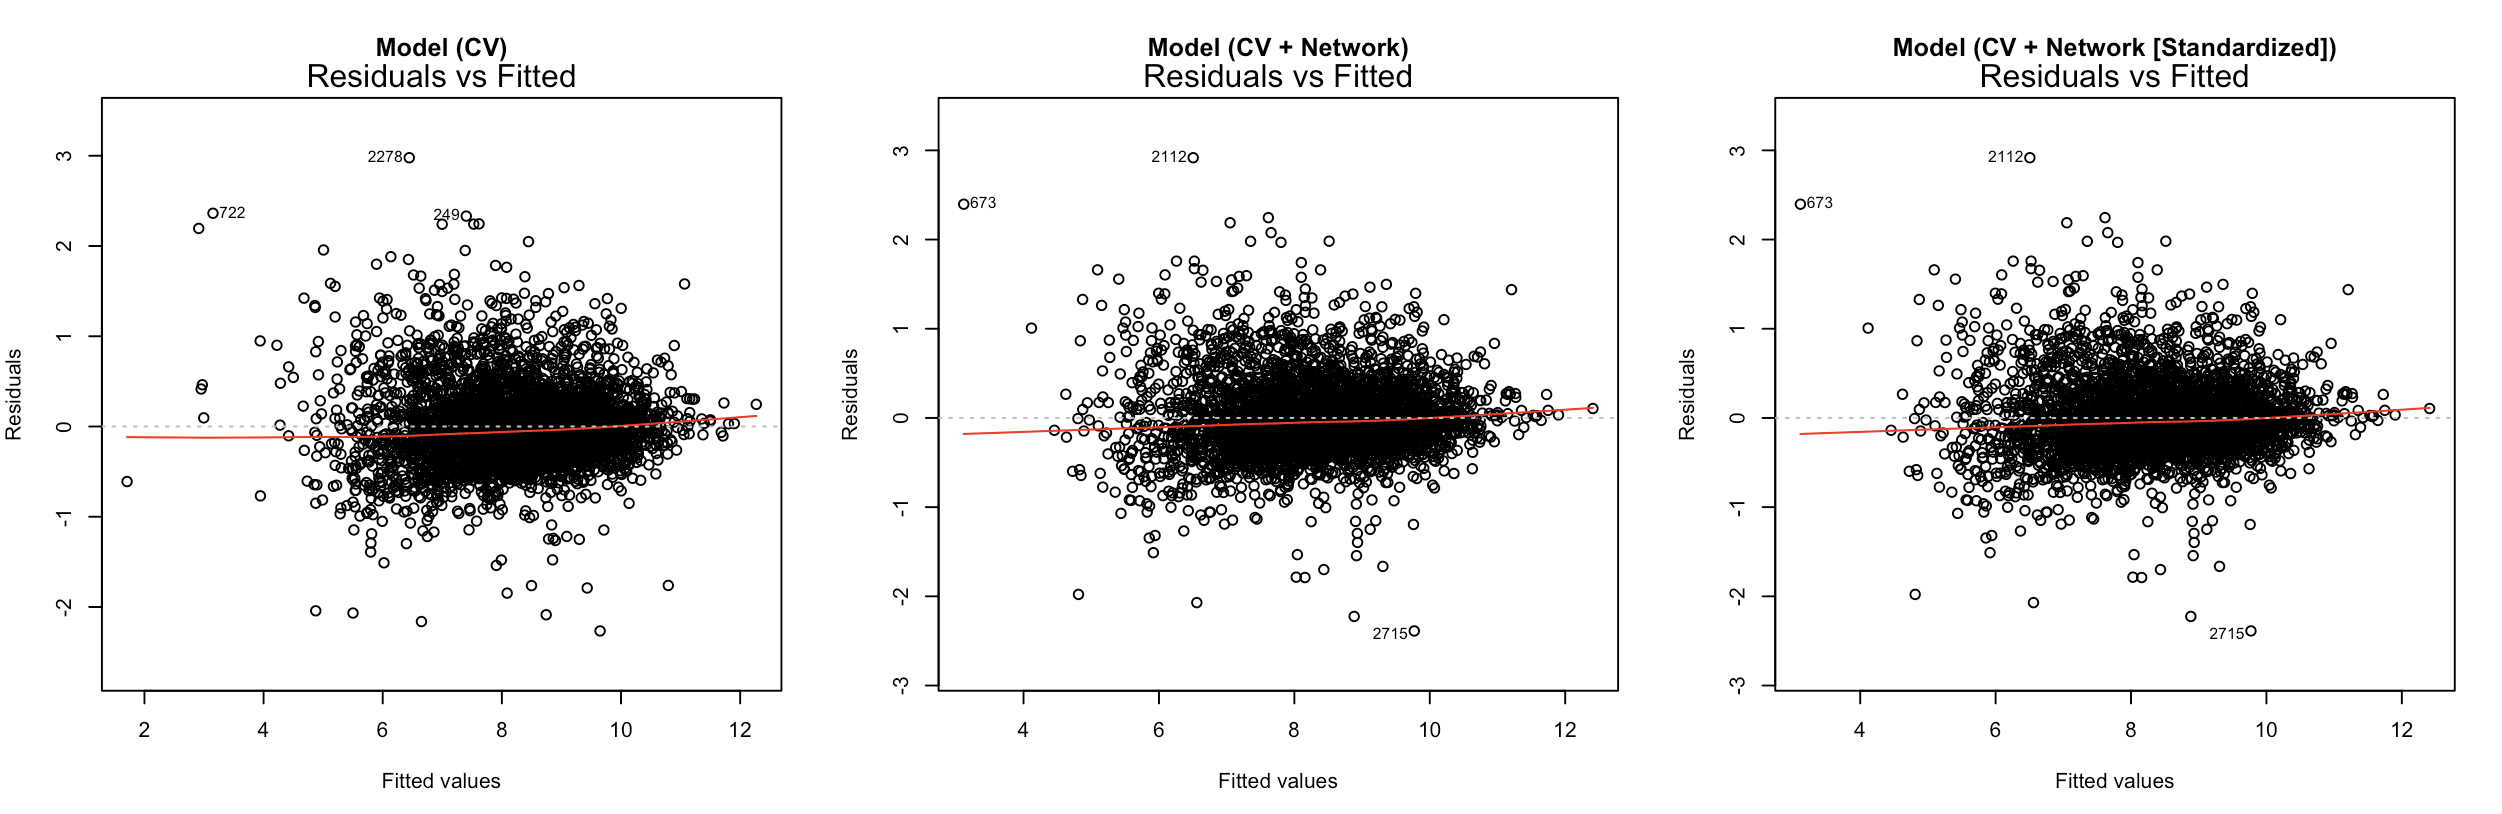
\includegraphics[scale=0.33]{ResidualPlots_TableS2.png}
    \end{center}
\end{description}

%Table S3
\newpage
\section*{\underline{Table S3:}}
\begin{table}[h!]
  \begin{center}
  \resizebox{\columnwidth}{!}{%
  \begin{tabular}{l l l l l l}
  
    \hline
    \hline
    
    {} & {(a)} & {(b)} & {(c)} & {(d)} & {(e)}  \\
    {} & {$\mathscr{C}^{PR}$} & {$\mathscr{C}^{B}$} & {$\mathscr{C}^{D}$} & {$\cancel{\beta_{N1},\beta_{N2}}$} & {$\cancel{\beta_{r}}$}  \\
    
    \hline
    
    \textbf {CV parameters}\\
    
    \rowcolor{gray!33}
    Departmental rank, $\beta_{r}$ 
    & -0.047*** & -0.042***  & -0.044*** & -0.046*** &         \\
    {} 
    & (0.006)   & (0.006)    & (0.006)   & (0.006)   &         \\
    
    \rowcolor{gray!33}
    Productivity (\textit{h}-index), $\beta_{h}$ 
    & 1.866***  & 1.901***   & 1.848***  & 1.862***  & 1.892*** \\
    {} 
    & (0.018)   & (0.019)    & (0.018)   & (0.018)   & (0.018)  \\
    
    \rowcolor{gray!33}
    Total NSF funding, $\beta_{\$1}$ 
    & -0.005*   & -0.004     & -0.005*   & -0.003**  & -0.005*  \\
    {} 
    & (0.002)   & (0.002)    & (0.002)   & (0.001)   & (0.002)  \\
    
    \rowcolor{gray!33}
    {\#} of NSF grants, $\beta_{N1}$ 
    & 0.013     & 0.009      & 0.007     &           & 0.006    \\
    {} 
    & (0.015)   & (0.015)    & (0.015)   &           & (0.015)  \\
    
    \rowcolor{gray!33}
    Total NIH funding, $\beta_{\$2}$ 
    & 0.014***  & 0.014***   & 0.014***  & 0.003*    & 0.013***  \\
    {} 
    & (0.003)   & (0.004)    & (0.003)   & (0.001)   & (0.004)   \\
    
    \rowcolor{gray!33}
    {\#} of NIH grants, $\beta_{N2}$ 
    & -0.061*** & -0.065***  & -0.062*** &           & -0.059**  \\
    {} 
    & (0.019)   & (0.020)    & (0.019)   &           & (0.019)   \\
    
    \hline
    
    \textbf {Network parameters}\\
    
    \rowcolor{gray!33}
    PageRank centrality, $\beta_{\mathscr{C}^{PR}}$ 
    & 0.041**  &            &            & 0.042**   & 0.057***  \\
    {} 
    & (0.014)  &            &            & (0.014)   & (0.014)   \\
    
    \rowcolor{gray!33}
    Betweenness centrality, $\beta_{\mathscr{C}^{B}}$ 
    &          & -0.000     &            &           &           \\
    {} 
    &          & (0.005)    &            &           &           \\
    
    \rowcolor{gray!33}
    Degree centrality, $\beta_{\mathscr{C}^{D}}$ 
    &          &            & 0.052***   &           &            \\
    {} 
    &          &            & (0.010)    &           &            \\
    
    \rowcolor{gray!33}
    Cross-disciplinarity, $\beta_{\chi}$ 
    & 0.571*** & 0.562***   & 0.530***   & 0.579***  & 0.555***    \\
    {} 
    & (0.061)  & (0.062)    & (0.061)    & (0.061)   & (0.061)     \\
    
    \hline
    
    \rowcolor{gray!33} 
    Discipline ($\mathscr{O}$) dummy & $\textit{Y}$ & $\textit{Y}$ & $\textit{Y}$ & $\textit{Y}$ & $\textit{Y}$ \\
    
    \rowcolor{gray!33} 
    5-year cohort $(y{^0_{i,5}})$ dummy & $\textit{Y}$ & $\textit{Y}$ & $\textit{Y}$ & $\textit{Y}$ & $\textit{Y}$ \\
    
    \rowcolor{gray!33} 
    Constant 
    & 1.706*** & 1.200***   & 1.344***   & 1.711***  & 1.615***  \\
    {} 
    & (0.271)  & (0.225)    & (0.226)    & (0.271)   & (0.273)   \\
    
    \hline
    
    \rowcolor{gray!33} 
    $\textit{n}$
    & 3900 & 3387 & 3900 & 3900 & 3900 \\
    
    \rowcolor{gray!33} 
    adj. ${R^2}$ 
    & 0.882 & 0.873 & 0.883 & 0.882 & 0.881 \\
    
    \hline
    \hline
    
    Standard errors in parentheses, & \multicolumn{5}{l}{listed below coefficient estimate.} \\
    {* $\textit{p}$ $\leq$ .05, ** $\textit{p}$ $\leq$ .01, *** $\textit{p}$ $\leq$ .001}
    
  \end{tabular}%
  }
  \end{center}
\end{table}
\begin{center}
\par{\textbf{Table S3. Career data set: Pooled cross-sectional model --- robustness check.}}
\end{center}
\newpage
\subsection*{\underline{Description of figure content:}}
\par{
The meaning of parameters and symbols are similar like Table S2. Here, the parameter estimates for the variants of the ‘CV + Network’ pooled cross-sectional models reported in Table S3: (a) Model with PageRank centrality ($df\$PRCentrality > 0$), (b) Model with betweenness centrality ($df\$BetCentrality > 0$), (c) Model with degree centrality ($df\$KDirect > 0$), (d) Model without the number of grants variables ($df\$PRCentrality > 0$), and (e) Model without the departmental rank variable ($df\$PRCentrality > 0$). The model (a) of the Table S3 is same as the (CV+Network) model of the Table S2. In next two models (b) and (c), the PageRank Centrality ($\mathscr{C}^{PR}$) has been replaced respectively by the Betweenness Centrality ($\mathscr{C}^{B}$) and the Degree Centrality ($\mathscr{C}^{D}$), those Betweenness and Degree Centrality are two alternative centrality along with the PageRank Centrality. In the model (d), the variables (${N^{NSF}}$ \& ${N^{NIH}}$) related to the number of grants have been removed. In the model (e), the department rank variable ($\beta_{r}$) has been removed. 
}
\subsection*{\underline{Observations, conclusions, and hypotheses:}}
\begin{description}
  \item In this Table S3, the robustness of the cross-sectional model has been tested by exploring several variations, through model (a) to (e). 
  \item[$\bullet$]  Model (a,b,c): The Betweenness and Degree Centrality are two alternative centrality along with the PageRank Centrality. Replacing the PageRank Centrality with those two centralities respectively doesn't indicate any significant differences.
  \item[$\bullet$]  Model (d): This model suspects the correlation effects, and so consider only the effect of total funding with removing the effect of number of grants. The result also isn't significantly different.
    \item[$\bullet$]  Model (e): This model assumes that the most recent university affiliation could inaccurately represent the career of faculties. The estimates after removing the department rank variable doesn't indicate any significant differences too.
    \item[$\bullet$] If we take a look at the significance level of estimate, then we can interpret that the department rank, $h-index$, NIH variables, and cross-disciplinarity are more significant to the model as $p-value$ is than 0.001. 
    \item[$\bullet$] Here, for model (a), observations = 3900 and Adjusted R-squared = 0.882 ($df\$PRCentrality > 0$); for model (b), observations = 3387 and Adjusted R-squared = 0.873 ($df\$BetCentrality > 0$); for model (c), observations = 3900 and Adjusted R-squared = 0.883 ($df\$KDirect > 0$); for model (d), observations = 3900 and Adjusted R-squared = 0.882 ($df\$PRCentrality > 0$); for model (e), observations = 3900 and Adjusted R-squared = 0.881 ($df\$PRCentrality > 0$). The R-squared value is large for all model (to be specific, model (b) is slightly larger than others) that indicates the data are closer to the fitted regression line for all model. 
    \item[$\bullet$] The residuals seems to be strongly randomly scattered for all model and it is almost linear line. Additionally, all the values of VIF (computed by $\textbf{car::vif(model\_x)}$) ensures that multicollinearity isn’t available here. Thus represents the goodness of the models. 
    \begin{center}
    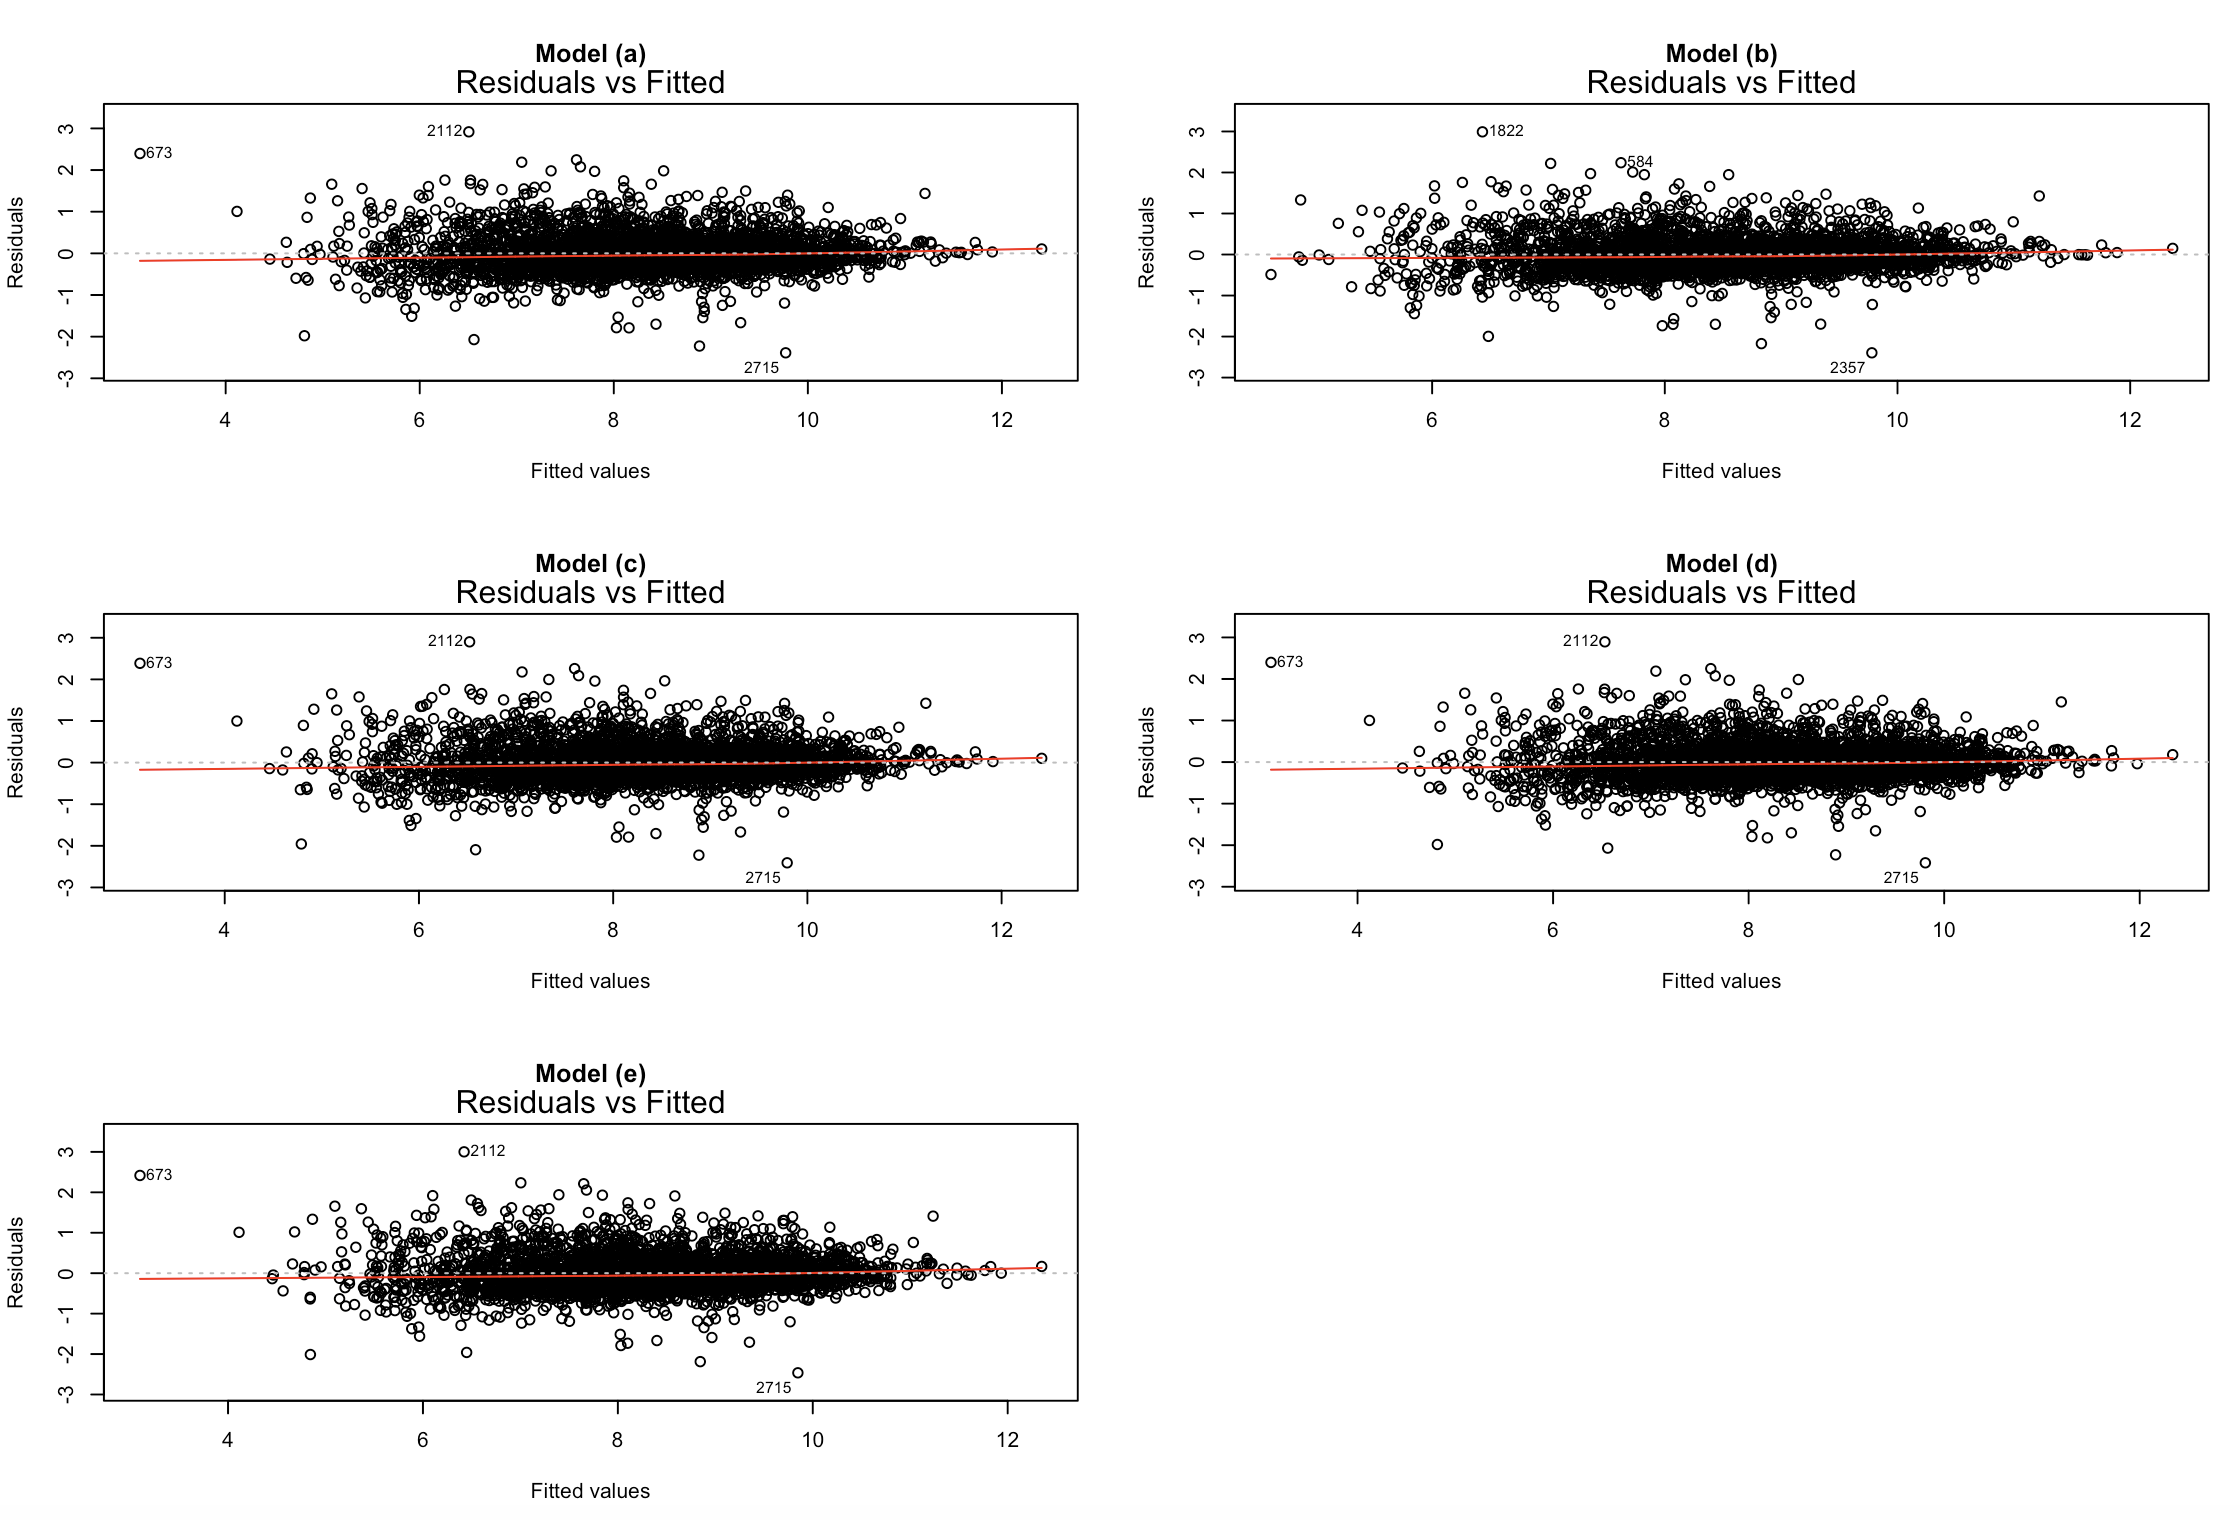
\includegraphics[scale=0.33]{ResidualPlots_TableS3.png}
    \end{center}
  \item Therefore, in all cases, the results of the modified regression estimates are not significantly different with respect to the primary covariate of interest (cross-disciplinarity ($\beta_{\chi}$)), thus indicates the robustness of the cross-sectional model.
\end{description}

\end{document}
